Using a low-rank \gls{SVD} approximation for the \gls{M2L} operator matrix
naturally leads to the question of what the optimum choice for target rank for $k$
is (see Chapter \ref{chpt:2_strategy_for_practical_implementation}, Section \ref{sec:2_4_svd_compression}).
Naturally, we want to minimise $k$ to reduce the asymptotic complexity of
the application of the compressed \gls{M2L} operator. However, it's clear that
if $k$ is taken to be too low, we will be losing potentially important data
from the original uncompressed \gls{M2L} matrix. However, if $k$ is too high
we will be keeping redundant singular vectors which do not contribute significantly
to the final result for potential.

For this experiment we use a 3 level octree containing 1000 randomly distributed
particles in a unit cube, which are taken to be sources as well as targets, and
with unit charges have been placed on the sources. We compute $p=3$ degree multipole and
local expansions therefore discretising each surface with 26 quadrature points.
Our metric is the mean percentage error of the \gls{PyExaFMM} result and
full-rank \gls{M2L} matrices, with respect to the direct result.
This mean is taken across errors for all target particles. For the above
tree topology and expansion order $p$, we find a a mean percentage error of
$1.96$ \% (2 d.p) when the \gls{M2L} matrix is left full-rank.
This experiment is repeated for different low-rank approximations,
the results of which are illustrated in figure (\ref{fig:3_2_svd}).

\begin{figure}[ht]
    \centering

  {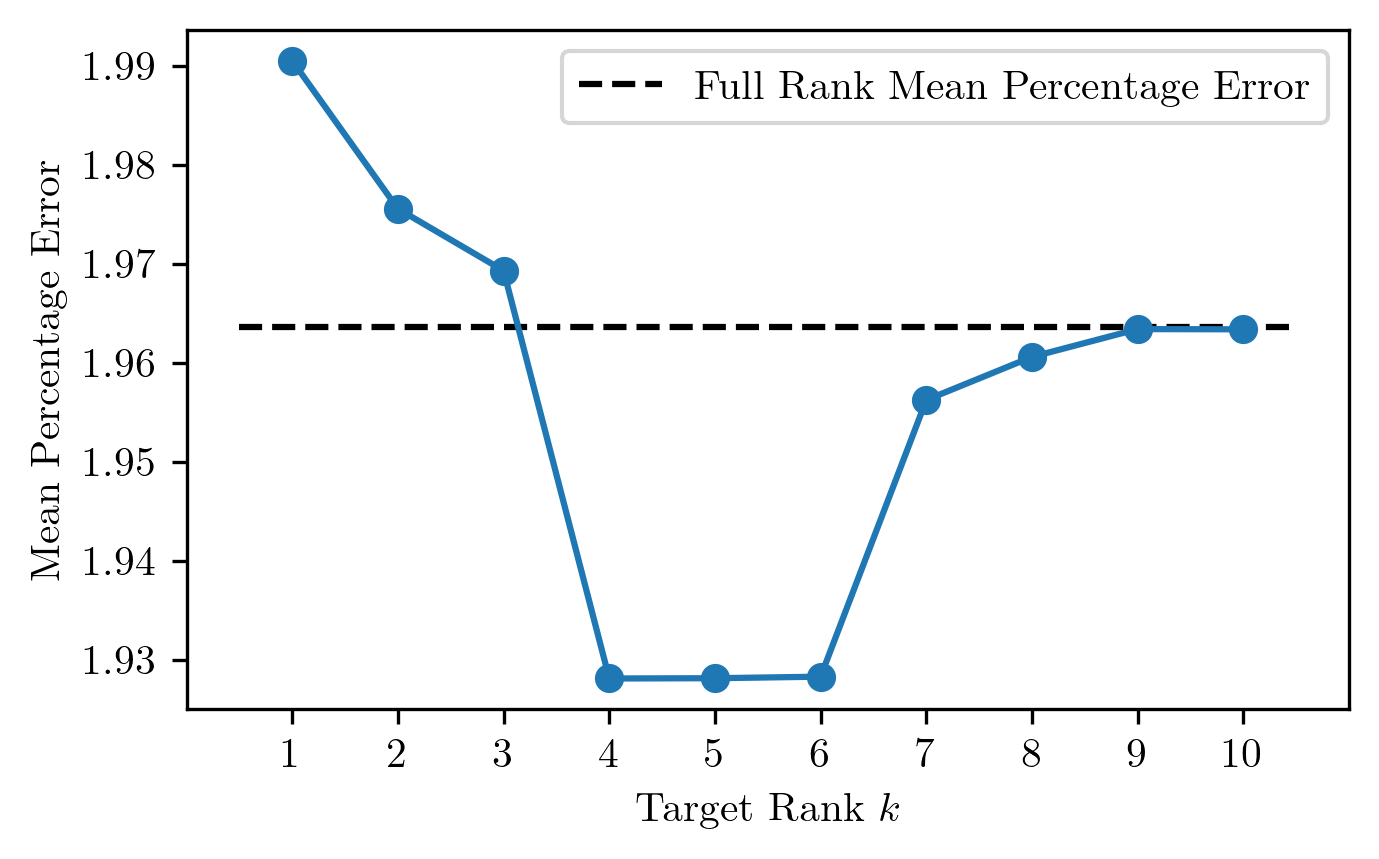
\includegraphics[width=0.9\textwidth]{chapter3/svd.png}}
  \vspace{0pt}
    \caption{Mean percentage error of \gls{PyExaFMM} with respect to direct
    computation, where the mean is taken across all particles in the simulation.
    The mean percentage error for the full-rank simulation is illustrated with
    a dashed horizontal line.
    }
    \label{fig:3_2_svd}
\end{figure}

Figure (\ref{fig:3_2_svd}) indicates that singular vectors corresponding to rank
greater than 6 are actually adding noise to the results of \gls{PyExaFMM}, with
an optimum target rank $k$ in the range 4-6 for the above tree topology. Currently
\gls{PyExaFMM} does not attempt to find an optimum rank for a given tree topology,
however this represents a future body of work.
